\documentclass{article}
\usepackage{fancyhdr}
\usepackage{amsthm}
\usepackage{etoolbox}
\usepackage{verbatim}
\usepackage{enumerate}
\usepackage{amsmath}
\usepackage{algorithmicx}
\usepackage{algorithm}
\usepackage{algpseudocode}
\usepackage{amssymb}
\usepackage{tikz}
	
\pagestyle{fancy}
\title{Chapter 21}
\author{Michelle Bodnar, Andrew Lohr}

\newcounter{curnum}
\setcounter{curnum}{0}

\newtheorem{th1}{Exercise} 
\newcommand{\calH}{\mathcal{H}}
\newcommand{\calX}{\mathcal{X}}
\newcommand{\calA}{\mathcal{A}}
\newcommand{\calY}{\mathcal{Y}}

\begin{document}
\maketitle


\noindent\textbf{Exercise 21.1-1}\\
$
\begin{array}{c|ccccccccccc}
Edge Processed&&&&&&&&&&&\\
\hline
initial&\{a\}&\{b\}&\{c\}&\{d\}&\{e\}&\{f\}&\{g\}&\{h\}&\{i\}&\{j\}&\{k\}\\
(d,i)&\{a\}&\{b\}&\{c\}&\{d,i\}&\{e\}&\{f\}&\{g\}&\{h\}&&\{j\}&\{k\}\\
(f,k)&\{a\}&\{b\}&\{c\}&\{d,i\}&\{e\}&\{f,k\}&\{g\}&\{h\}&&\{j\}&\\
(g,i)&\{a\}&\{b\}&\{c\}&\{d,i,g\}&\{e\}&\{f,k\}&&\{h\}&&\{j\}&\\
(b,g)&\{a\}&\{b,d,i,g\}&\{c\}&&\{e\}&\{f,k\}&&\{h\}&&\{j\}&\\
(a,h)&\{a,h\}&\{b,d,i,g\}&\{c\}&&\{e\}&\{f,k\}&&&&\{j\}&\\
(i,j)&\{a,h\}&\{b,d,i,g,j\}&\{c\}&&\{e\}&\{f,k\}&&&&&\\
(d,k)&\{a,h\}&\{b,d,i,g,j,f,k\}&\{c\}&&\{e\}&&&&&&\\
(b,j)&\{a,h\}&\{b,d,i,g,j,f,k\}&\{c\}&&\{e\}&&&&&&\\
(d,f)&\{a,h\}&\{b,d,i,g,j,f,k\}&\{c\}&&\{e\}&&&&&&\\
(g,j)&\{a,h\}&\{b,d,i,g,j,f,k\}&\{c\}&&\{e\}&&&&&&\\
(a,e)&\{a,h,e\}&\{b,d,i,g,j,f,k\}&\{c\}&&&&&&&&\\
\end{array}
$

So, the connected components that we are left with are $\{a,h,e\}$, $\{b,d,i,g,j,f,k\}$, and $\{c\}$.\\

\noindent\textbf{Exercise 21.1-3}\\
Find set is called twice on line 4, this is run once per edge in the graph, so, we have that find set is run $2|E|$ times. Since we start with $|V|$ sets, at the end only have $k$, and each call to UNION reduces the number of sets by one, we have that we have to of made $|V|-k$ calls to UNION.\\


\noindent\textbf{Exercise 21.2-1}\\
The three algorithms follow the english description and are provided here. There are alternate versions using the weighted union heuristic, suffixed with WU.
\begin{algorithm}
\caption{MAKE-SET(x)}
\begin{algorithmic}
\State Let o be an object with three fields, next, value, and set
\State Let L be a linked list object with head = tail = o
\State o.next = NIL
\State o.set = L
\State o.value = x
\State \Return L
\end{algorithmic}
\end{algorithm}
\begin{algorithm}
\caption{FIND-SET(x)}
\begin{algorithmic}
\State \Return o.set.head.value
\end{algorithmic}
\end{algorithm}
\begin{algorithm}
\caption{UNION(x,y)}
\begin{algorithmic}
\State L1= x.set
\State L2 = y.set
\State L1.tail.next = L2.head
\State z = L2.head
\While{$z.next \neq NIL$}
\State z.set = L1
\EndWhile
\State L1.tail = L2.tail
\State \Return L1
\end{algorithmic}
\end{algorithm}
\begin{algorithm}
\caption{MAKE-SET-WU(x)}
\begin{algorithmic}
\State L = MAKE-SET(x)
\State L.size = 1
\State \Return L
\end{algorithmic}
\end{algorithm}
\begin{algorithm}
\caption{UNION-WU(x,y)}
\begin{algorithmic}
\State L1= x.set
\State L2 = y.set
\If{$L1.size \ge L2.size$}
\State L =  UNION(x,y)
\Else
\State L =  UNION(y,x)
\EndIf
\State L.size = L1.size + L2.size
\State \Return L
\end{algorithmic}
\end{algorithm}

\noindent\textbf{Exercise 21.2-3}\\
During the proof of theorem 21.1, we concluded that the time for the $n$ UNION operations to run was at most $O(n\lg(n))$. This means that each of them took an ammortized time of at most $O(\lg(n))$. Also, since there is only a constant actual amount of work in performing MAKE-SET and FIND-SET operations, and none of that ease is used to offest costs of UNION operations, they both have $O(1)$ runtime.\\

\noindent\textbf{Exercise 21.2-5}\\
For each member of the set, we will make its first field which used to point back to the set object point instead to the last element of the linked list. Then, given any set, we can find its last element by going ot the head and following the pointer that that object maintains to the last element of the linked list. This only requires following exactly two pointers, so it takes a constant amount of time. Some care must be taken when unioning these modified sets. Since the set representative is the last element in the set, when we combine two linked lists, we place the smaller of the two sets before the larger, since we need to update their set represnetative pointers, unlike the original situation, where we update the representative of the objects that are placed on to the end of the linked list.\\

\noindent\textbf{Exercise 21.3-1}\\
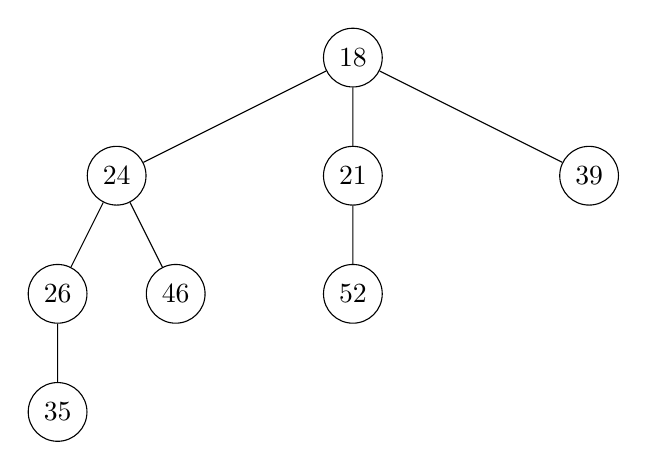
\begin{tikzpicture}[level/.style={sibling distance=30mm/#1}]
\node [circle,draw] (a){18}
  child{
node [circle,draw] (e){24}
  child {
  node [circle,draw] (f) {26}
  child{
  node [circle,draw] (g) {35}
  }
  }
  child {
  node [circle,draw] (h) {46}
  }
    }
  child {
  node [circle,draw] (b) {21}
  child{
  node [circle,draw] (c) {52}
  }
  }
  child {
  node [circle,draw] (d) {39}
  }
;
\end{tikzpicture}

\noindent\textbf{Exercise 21.3-3}\\
Suppose that $n' =2^k$ is the smallest power of two less than $n$. To see that this sequences of operations does take the required amount of time, we'll first note that after each iteration of the for loop indexed by j, we have that the elements $x_1,\ldots,x_{n'}$ are in trees of depth $i$. So, after we finish the outer for loop, we have that $x_1 \ldots x_{n'}$ all lie in the same set, but are represented by a tree of depth $k\in \Omega(\lg(n))$. Then, since we repeatedly call FIND-SET on an item that is $\lg(n)$ away from its set representative, we have that each one takes time $\lg(n)$. So, the last for loop alltogther takes time $m\lg(n)$.\\
\begin{algorithm}
\caption{Sequence of operations for Exercise 21.3-3}
\begin{algorithmic}
\For{i=1..n}
\State MAKE-SET{$x_i$}
\EndFor
\For{$i=1..k$}
\For{$j=1 .. n'-2^{i=1} by 2^{i}$}
\State UNION($x_i$,$x_{i+2^{j-1}}$)
\EndFor
\EndFor
\For{$i=1..m$}
\State FIND-SET($x_1$)
\EndFor
\end{algorithmic}
\end{algorithm}

\noindent\textbf{Exercise 21.3-5}\\
Clearly each MAKE-SET and LINK operation only takes time $O(1)$, so, supposing that n is the number of FIND-SET operations occuring after the making and linking, we need to show that all the FIND-SET operations only take time $O(n)$. To do this, we will ammortize some of the cost of the FIND-SET operations into the cost of the MAKE-SET operations. Imagine paying some constant amount extra for each MAKE-SET operation. Then, when doing a FIND-SET(x) operation, we have three possibilities. First, we could have that $x$ is the representative of its own set. In this case, it clearly only takes constant time to run. Second, we could have that the path from x to its set's representative is already compressed, so it only takes a single step to find the set representative. In this case also, the time required is constant. Lastly, we could have that x is not the representative and it's path has not been compressed. Then, suppose that there are $k$ nodes between $x$ and its representative. The time of this find-set operation is $O(k)$, but it also ends up compressing the paths of $k$ nodes, so we use that extra amount that we paid during the MAKE-SET operations for these $k$ nodes whoose paths were compressed. Any subsequent call to find set for these nodes will take only a constant amount of time, so we would nver try to use the work that ammortization amount twice for a given node.\\

\noindent\textbf{Exercise 21.4-1}\\
The initial value of x.rank is 0, as it is initialized in line 2 of the MAKE-SET(x) procedure. When we run LINK(x,y), whichever one has the larger rank is placed as the parent of the other, and if there is a tie, the parent's rank is incremented. This means that after any LINK(y,x), the two nodes being linked satisfy this strict inequality of ranks. Also, if we have that $x\neq x.p$, then, we have that $x$ is not its own set representative, so, any linking together of sets that would occur would not involve $x$, but that's the only way for ranks to increase, so, we have that x.rank must remain constant after that point.\\


\noindent\textbf{Exercise 21.4-3}\\
Since their value is at most $\lfloor \lg(n)\rfloor$, we can represent them using $\Theta(\lg(\lg(n)))$ bits, and may need to use that many bits to represent a number that can take that many values.\\

\noindent\textbf{Exercise 21.4-5}\\
He isn't correct, suppose that we had that $rank(x.p) >A_{2}(rank(x))$ but that $rank(x.p.p) = 1 + rank(x.p)$, then we would have that $level(x.p) =0$, but $level(x) \ge 2$. So, we don't have that $level(x) \le level(x.p)$ even though we have that the ranks are monotonically increasing as we go up in the tree. Put another way, even though the ranks are monotonically increasing, the rate at which they are increasing (roughly captured by the level vales) doesn't have to, itself be increasing.\\ 

\noindent\textbf{Problem 21-1}\\
\begin{enumerate}[a.]
\item
$
\begin{array}{|c|c|}
\hline
index&value\\
\hline
1&4\\
2&3\\
3&2\\
4&6\\
5&8\\
6&1\\
\hline
\end{array}
$

\item
As we run the for loop, we are picking off the smallest of the possible elements to be removed, knowing for sure that it will be removed by the next unused EXTRACT-MIN operation. Then, since that EXTRACT-MIN operation is used up, we can pretend that it no longer exists, and combine the set of things that were inserted by that segment with those inserted by the next, since we know that the EXTRACT-MIN operation that had separated the two is now used up. Since we proceed to figure out what the various extract operations do one at a time, by the time we are done, we have figured them all out.

\item
We let each of the sets be represented by a disjoint set structure. To union them (as on line 6) just call UNION. Checking that they exist is just a matter of keeping track of a linked list of which ones exist(needed for line 5), initially containing all of them, but then, when deleting the set on line 6, we delete it from the linked list that we were maintaining. The only other interation with the sets that we have to worry about is on line 2, which just amounts to a call of FIND-SET(j). Since line 2 takes ammorized time $\alpha(n)$ and we call it exactly $n$ times, then, since the rest of the for loop only takes constant time, the total runtime is $O(n\alpha(n))$.

\end{enumerate}

\noindent\textbf{Problem 21-3}\\
\begin{enumerate}[a.]
\item

Suppose that we let $\le_{LCA}$ to be an ordering on the vertices so that $u\le_{LCA} v$ if we run line 7 of $LCA(u)$ before line 7 of $LCA(v)$. Then, when we are running line 7 of $LCA(u)$, we immeduatle go on to the for loop on line 8. So, while we are doing this for loop, we still haven't called line 7 of LCA(v). This means that v.color is white, and so, the pair \{u,v\} is not considered during the run of LCA(u). However, during the for loop of LCA(v), since line 7 of LCA(u) has already run, u.color = black. This means that we will consider the pair \{u,v\} during the running of LCA(v).

It is not obvious what the ordering $\le_{LCA}$ is, as it will be implementation dependent. It depends on the order in which child vertices are iterated in the for loop on line 3. That is, it doesn't just depend on the graph structure.

\item
We suppose that it is true prior to a given call of $LCA$, and show that this property is preserved throughout a run of the procedure, increasing the number of disjoint sets by one by the end of the procedure. So, supposing that $u$ has depth $d$ and there are $d$ items in the disjoint set datastructure before it runs, it increases to d+1 disjoint sets on line 1. So, by the time we get to line 4, and call LCA of a child of $u$, there are d+1 disjoint sets, this is exactly the depth of the child. After line 4, there are now $d+2$ disjoint sets, so, line 5 brings it back down to $d+1$ disjoint sets for the subsequent times through the loop. After the loop, there are no more changes to the number of disjoint sets, so, the algorithm terminates with d+1 disjoint sets, as desired. Since this holds for any arbitrary run of LCA, it holds for all runs of LCA.

\item
Suppose that the pair $u$ and $v$ have the least common ancestor $w$. Then, when running $LCA(w)$, u will be in the subtree rooted at one of $w$'s children, and $v$ will be in another. WLOG, suppose that the subtree containing $u$ runs first. So, when we are done with running that subtree, all of their ancestor values will point to $w$ and their colors will be black, and their ancestor values will not change until $LCA(w)$ returns. However, we run LCA(v) before $LCA(w)$ returns, so in the for loop on line 8 of LCA(v), we will be considering the pair $\{u,v\}$, since $u.color==BLACK$. Since u.ancestor is still $w$, that is what will be output, which is the correct answer for their LCA.

\item
The time complexity of lines 1 and 2 are just constant. Then, for each child, we have a call to the same procedure, a UNION operation which only takes constant time, and a FIND-SET operation which can take at most ammortized inverse Ackerman's time. Since we check each and every thing that is adjacent to $u$ for being black, we are only checking each pair in $P$ at most twice in lines 8-10, among all the runs of $LCA$. This means that the total runtime is $O(|T| \alpha(|T|) + |P|)$.

\end{enumerate}


\end{document}